%KASCADE gamma search

% \begin{frame}{KASCADE-Grande}
% \begin{itemize}
%   \item Proposed in 1989---disassembled in 2013;
%   \item Aimed at studying
%   high-evergy (galactic) cosmic rays by observing extensive air showers (EAS);
% %   processes at the edge of the Galaxy and beyond by observing extended atmospheric showers (EAS);
%   \item Consisted of:
%   \begin{itemize}
%     \item scintillators detecting $e$, $\gamma$, $\mu$:
%     \begin{itemize}
%   %сцинтиляторы, различают e, gamma, mu
%     \item KASCADE---256 stations;
%     \item GRANDE---37 stations;
%     \end{itemize}
%  %один большой калориметр
%     \item Hadronic callorimeter;
%  %радиодетектор
%     \item Digital radio array LOPES detecting $e$, $e^{+}$;
% % позволяющих наблюдать различные компоненты ливня
%   \end{itemize}
%   \item Important features of cosmic-ray spectrum have been obtained. The data analysis is ongoing;
% %  благодаря данным с эксперимента было открыто много всего ополезного, при этом анлиз данных продолжается. новые статьи выходят
%   \item KCDC (\textbf{K}ASCADE \textbf{C}osmic Ray \textbf{D}ata \textbf{C}enter, \textcolor{blue}{\texttt{http://kcdc.ikp.kit.edu}}) is a dedicated portal where all the data collected are available online. % At the moment
% \end{itemize}
% 
% \begin{frame}{KASCADE-Grande gamma-ray limits}
% %   \item Limits on the ratio of diffuse gamma-ray flux to cosmic ray flux
%   \begin{minipage}{0.5\textwidth}
%    left
%   \end{minipage}
% 
% %   \begin{columns}
% %     \column{0.5\textwidth}
% %     left
% %     \column{0.5\textwidth}
% %     right
% %   \end{columns}
% \end{frame}


\section{KASCADE high-energy \texorpdfstring{$\gamma$}{gamma}-ray search}

\begin{frame}{KASCADE experiment}
\begin{itemize}
\item Location: 110~m a.s.l., 49$^\circ$N, 8$^\circ$E, KIT-Campus North, Karlsruhe, Germany;
\end{itemize}
\vspace{-\itemsep}
\begin{minipage}[c]{0.5\textwidth}
\begin{itemize}
\item Operation time:\\1996 October -- 2010 May $\Rightarrow$ effective time $\sim 4223.6$ days;
\item Area: $200 \times 200$ m$^2$;
\item 252 scintillator detectors;
\item $N_e$ ($> 5$~MeV);
\item $N_{tr \mu}$ ($> 230$~MeV, $r = 40 - 200$~m).
\end{itemize}
\end{minipage}\hfill
\begin{minipage}[c]{0.49\textwidth}
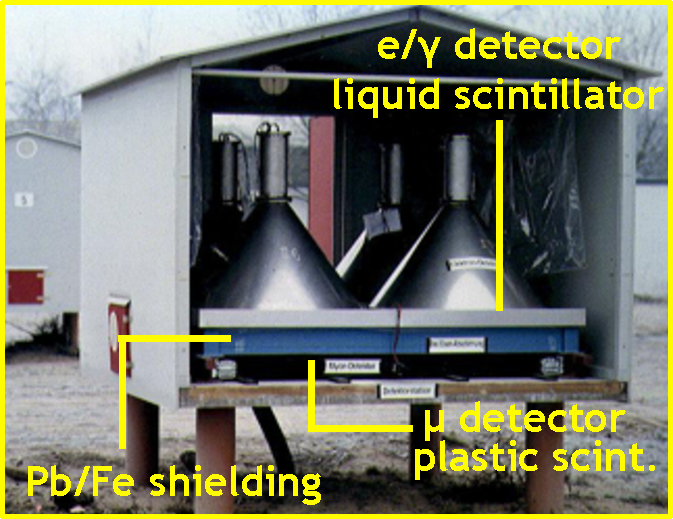
\includegraphics[width=1\textwidth]{pics/KASCADE-station.pdf}
\end{minipage}
\end{frame}

\begin{frame}{High-energy $\gamma$-ray sources in KASCADE field of view}
%   KASCADE data: Efficiency of registration, exposure map *
\begin{minipage}[c]{0.73\textwidth}
\begin{center}
  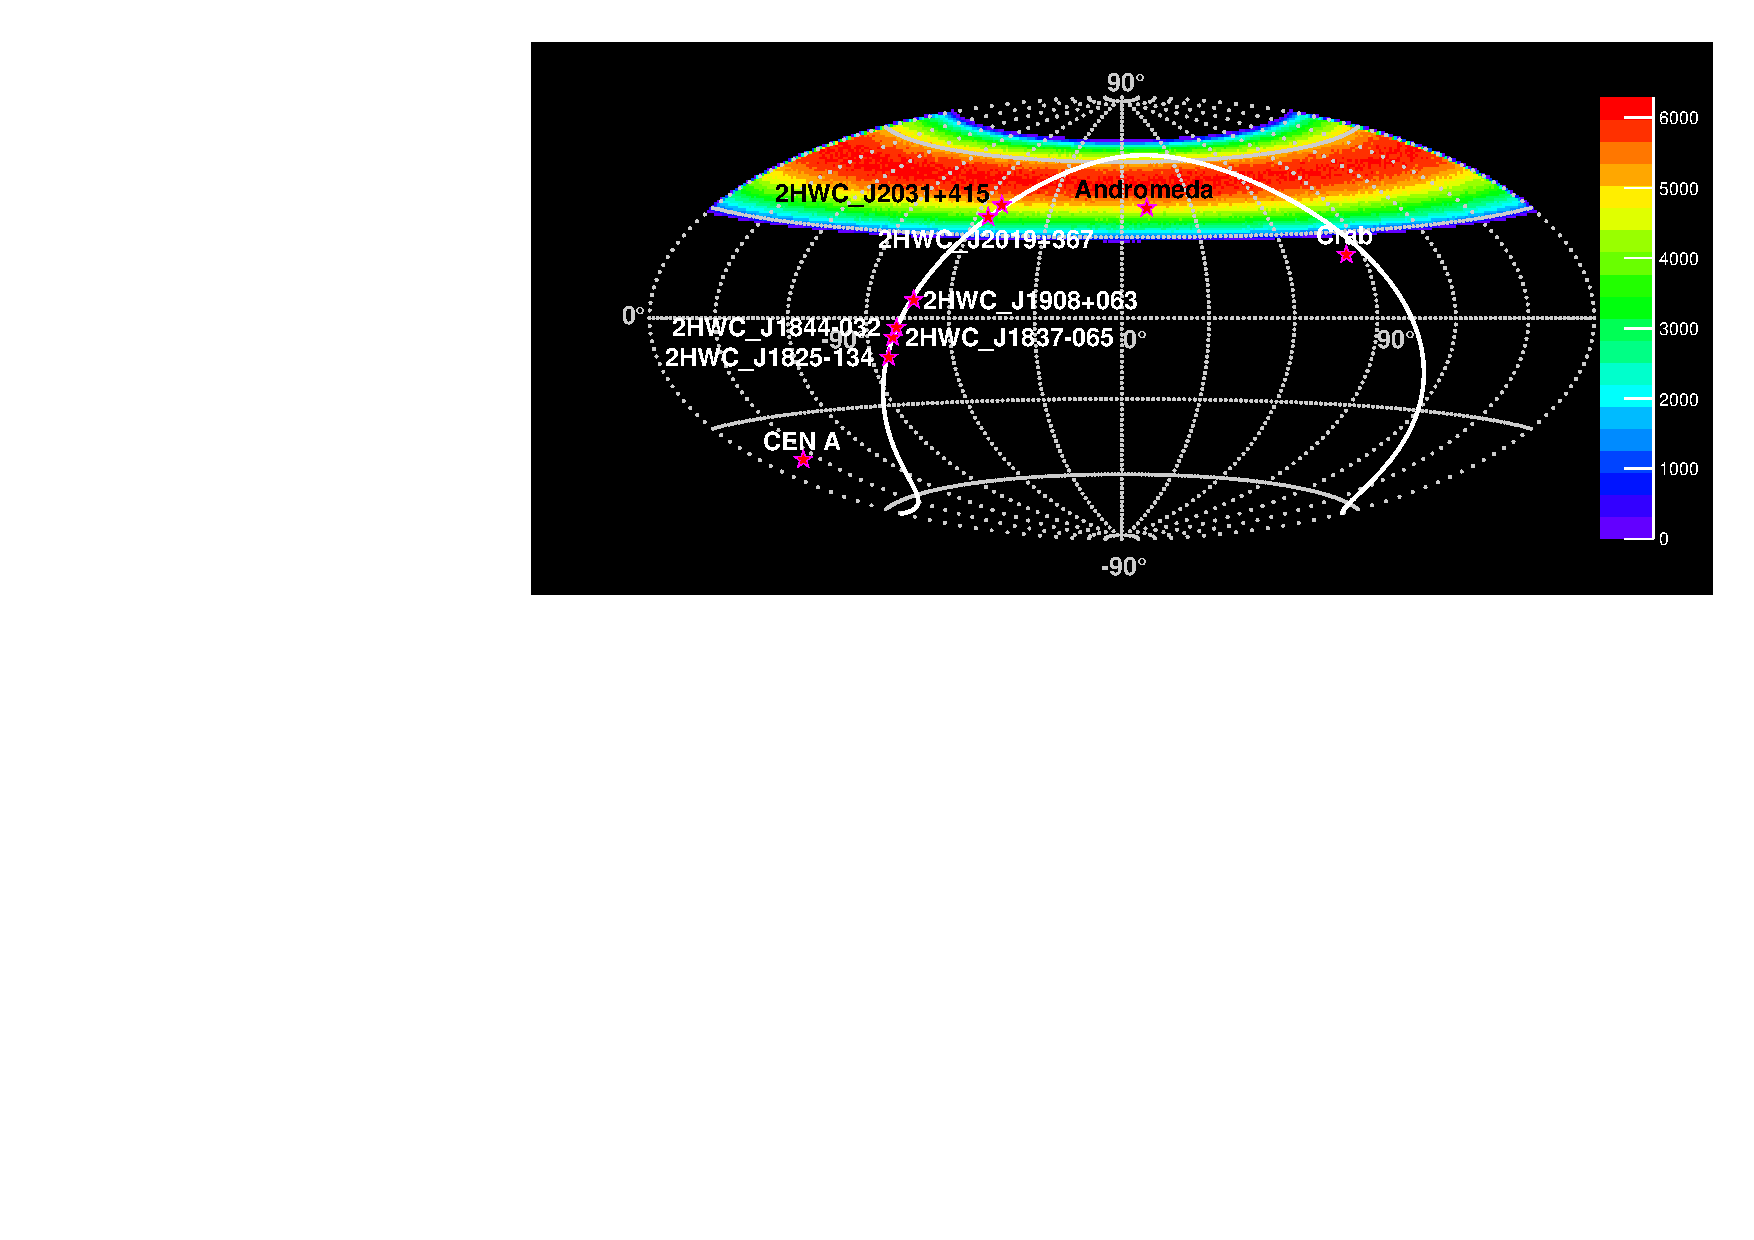
\includegraphics[width=1\textwidth]{pics/Skymap_6srcs.pdf}\\
  KASCADE event distribution map\\
  with 6 HAWC sources\\
  with energy $E$ above 56~TeV.
\end{center}
\end{minipage}
\hfill
\begin{minipage}[c]{0.25\textwidth}
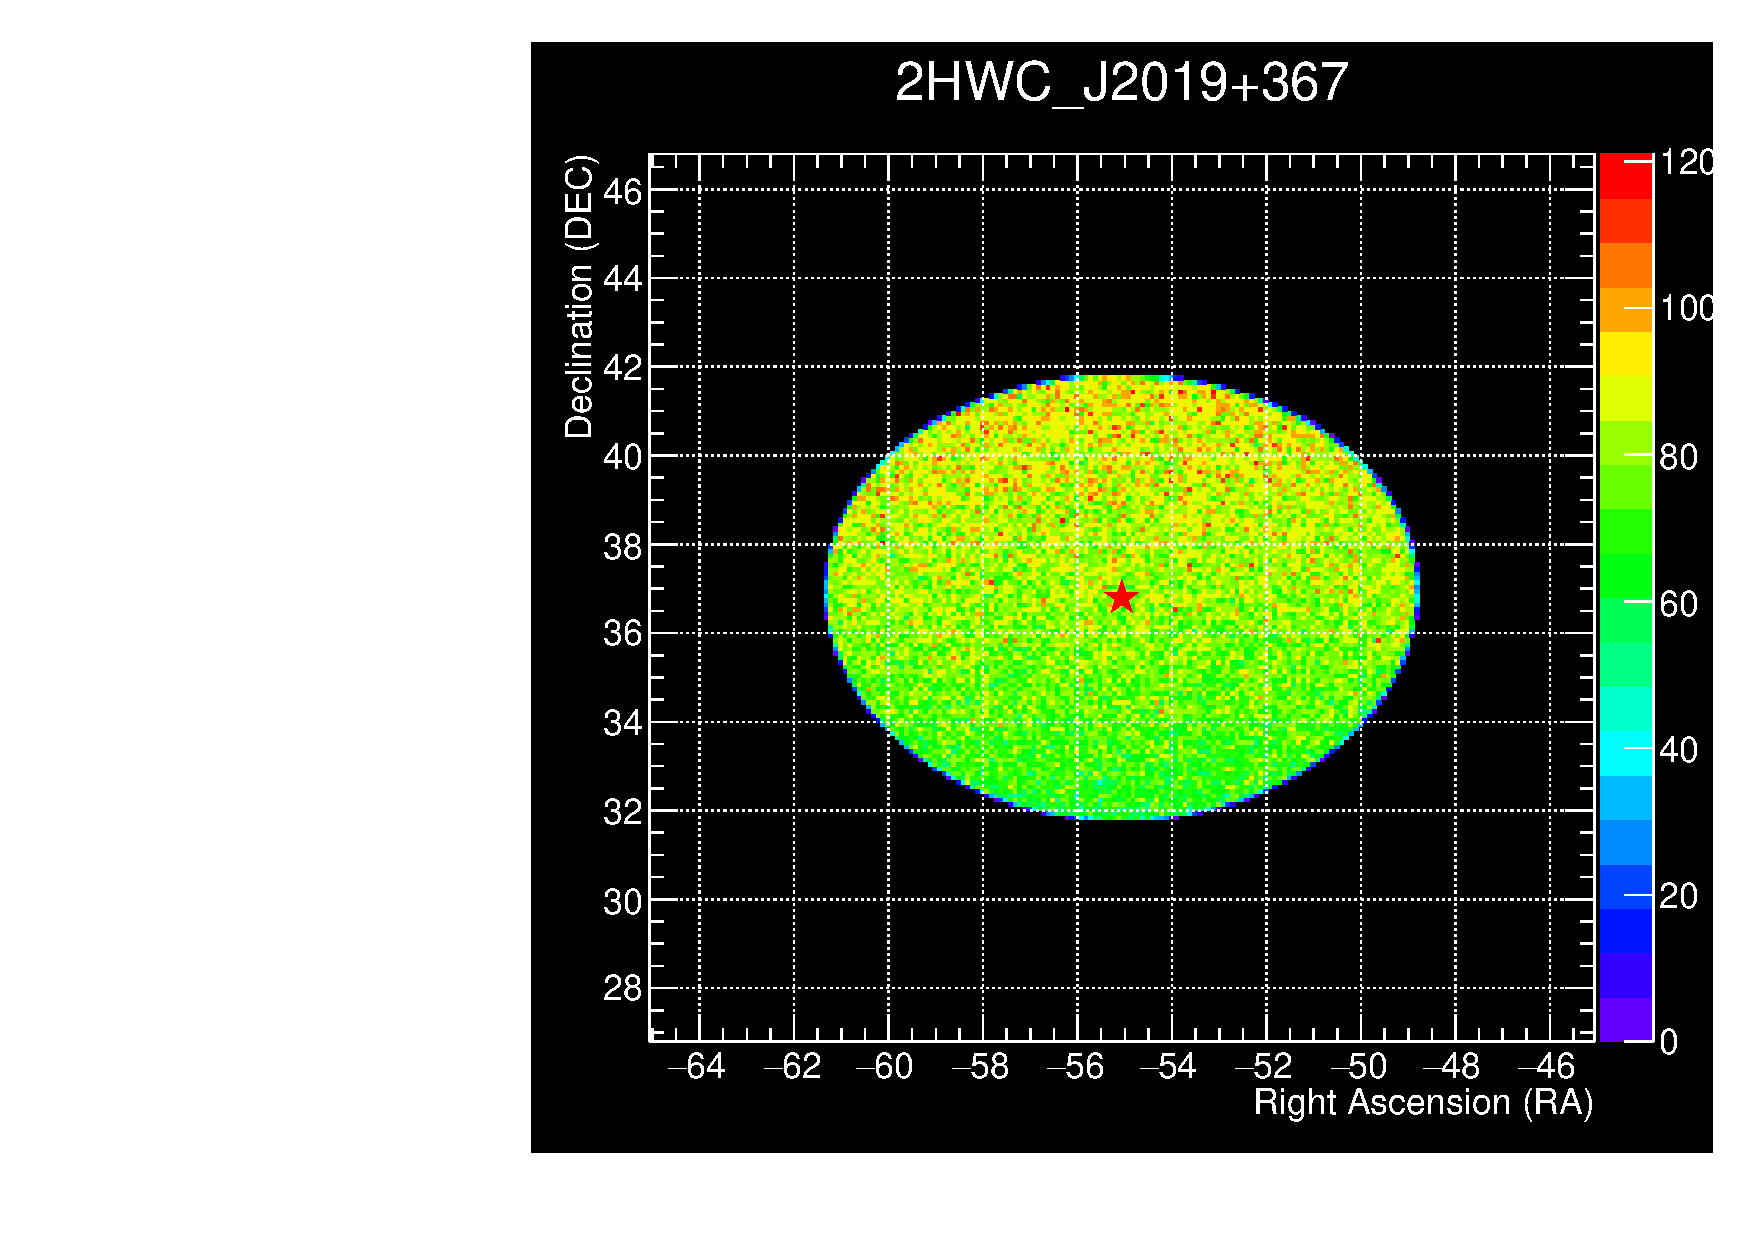
\includegraphics[width=1\textwidth]{pics/Skymap_2HWC_J2019+367.pdf}\\
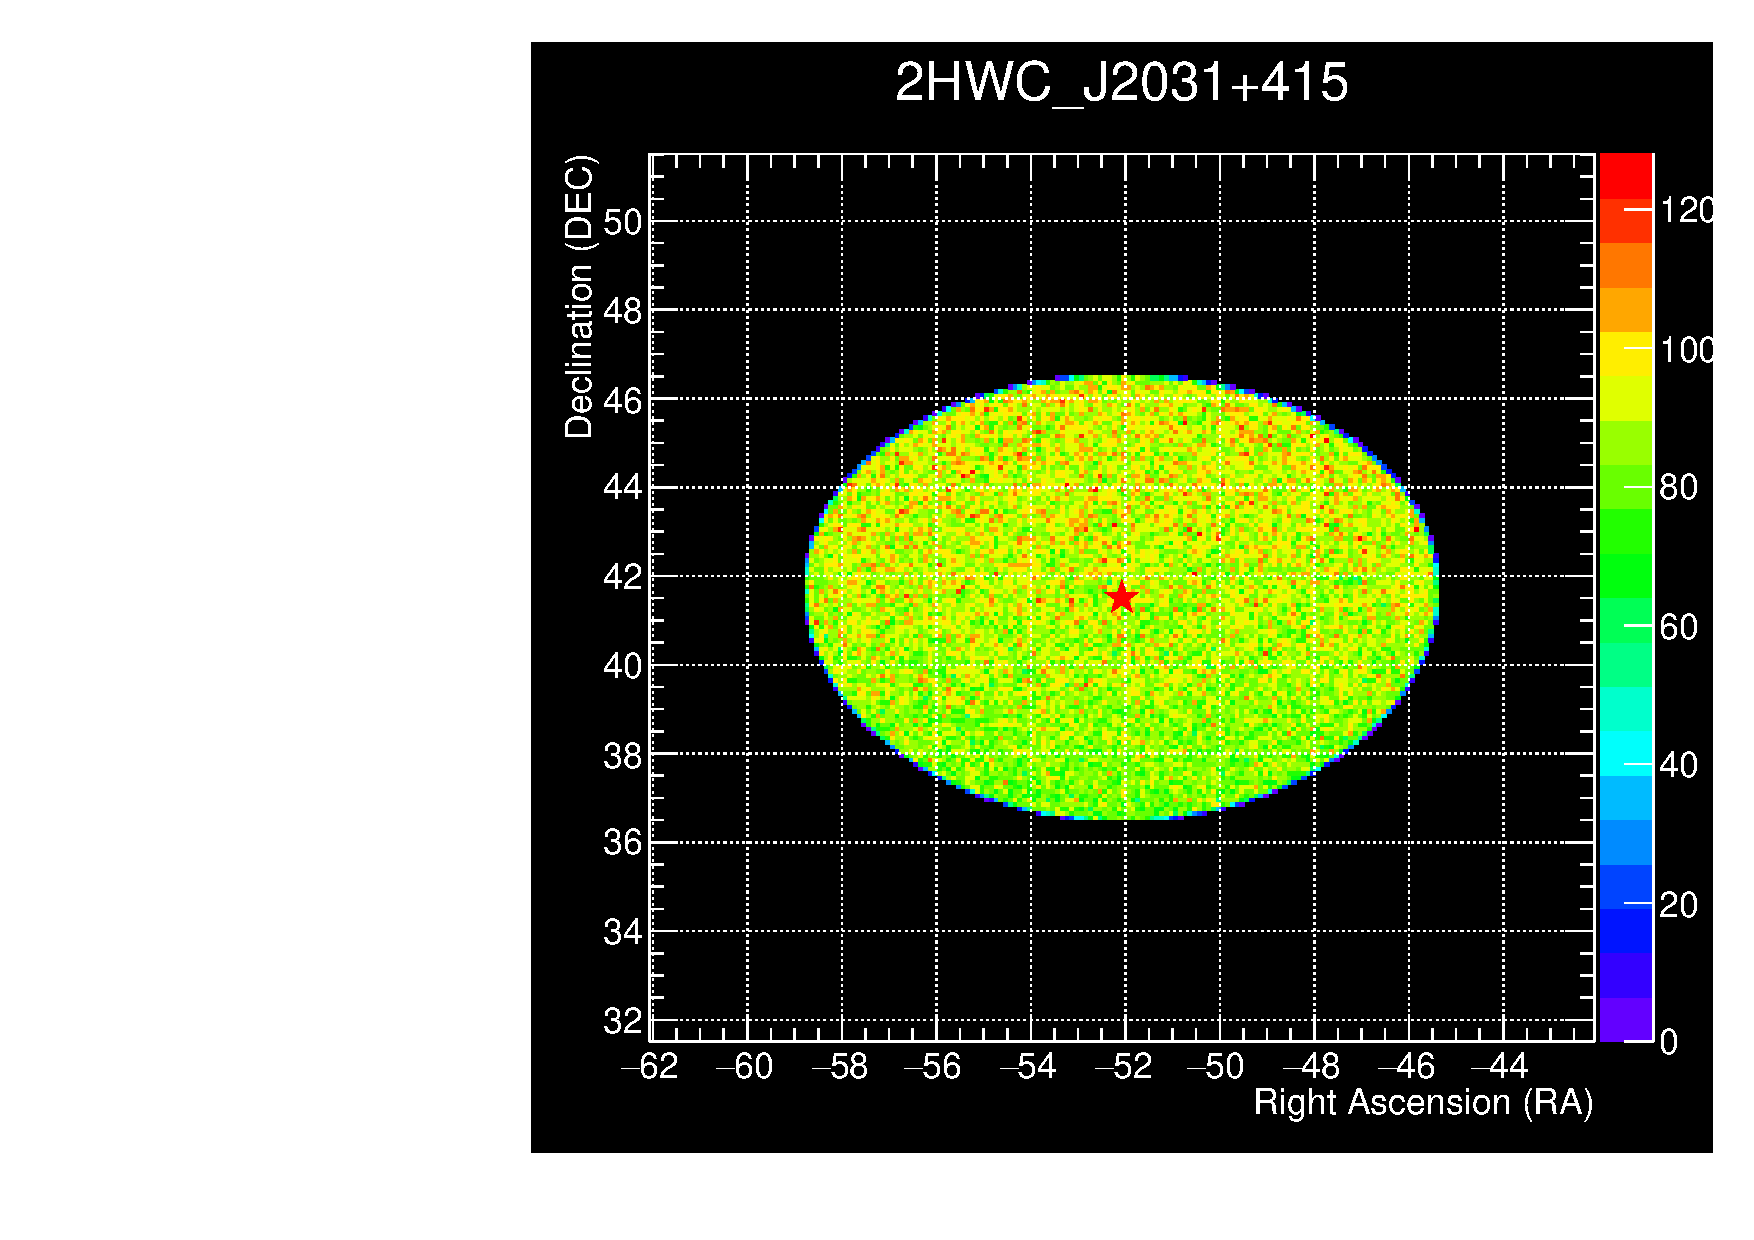
\includegraphics[width=1\textwidth]{pics/Skymap_2HWC_J2031+415.pdf}
\end{minipage}
\end{frame}

\begin{frame}{Data cuts and corrections}
\begin{center}
  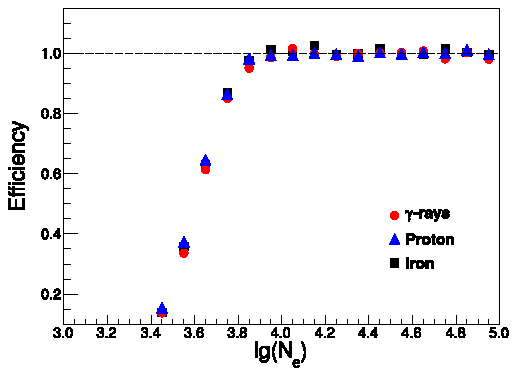
\includegraphics[height=0.39\textheight]{pics/eff_Ne_Donghwa.pdf}\hspace{1em}
  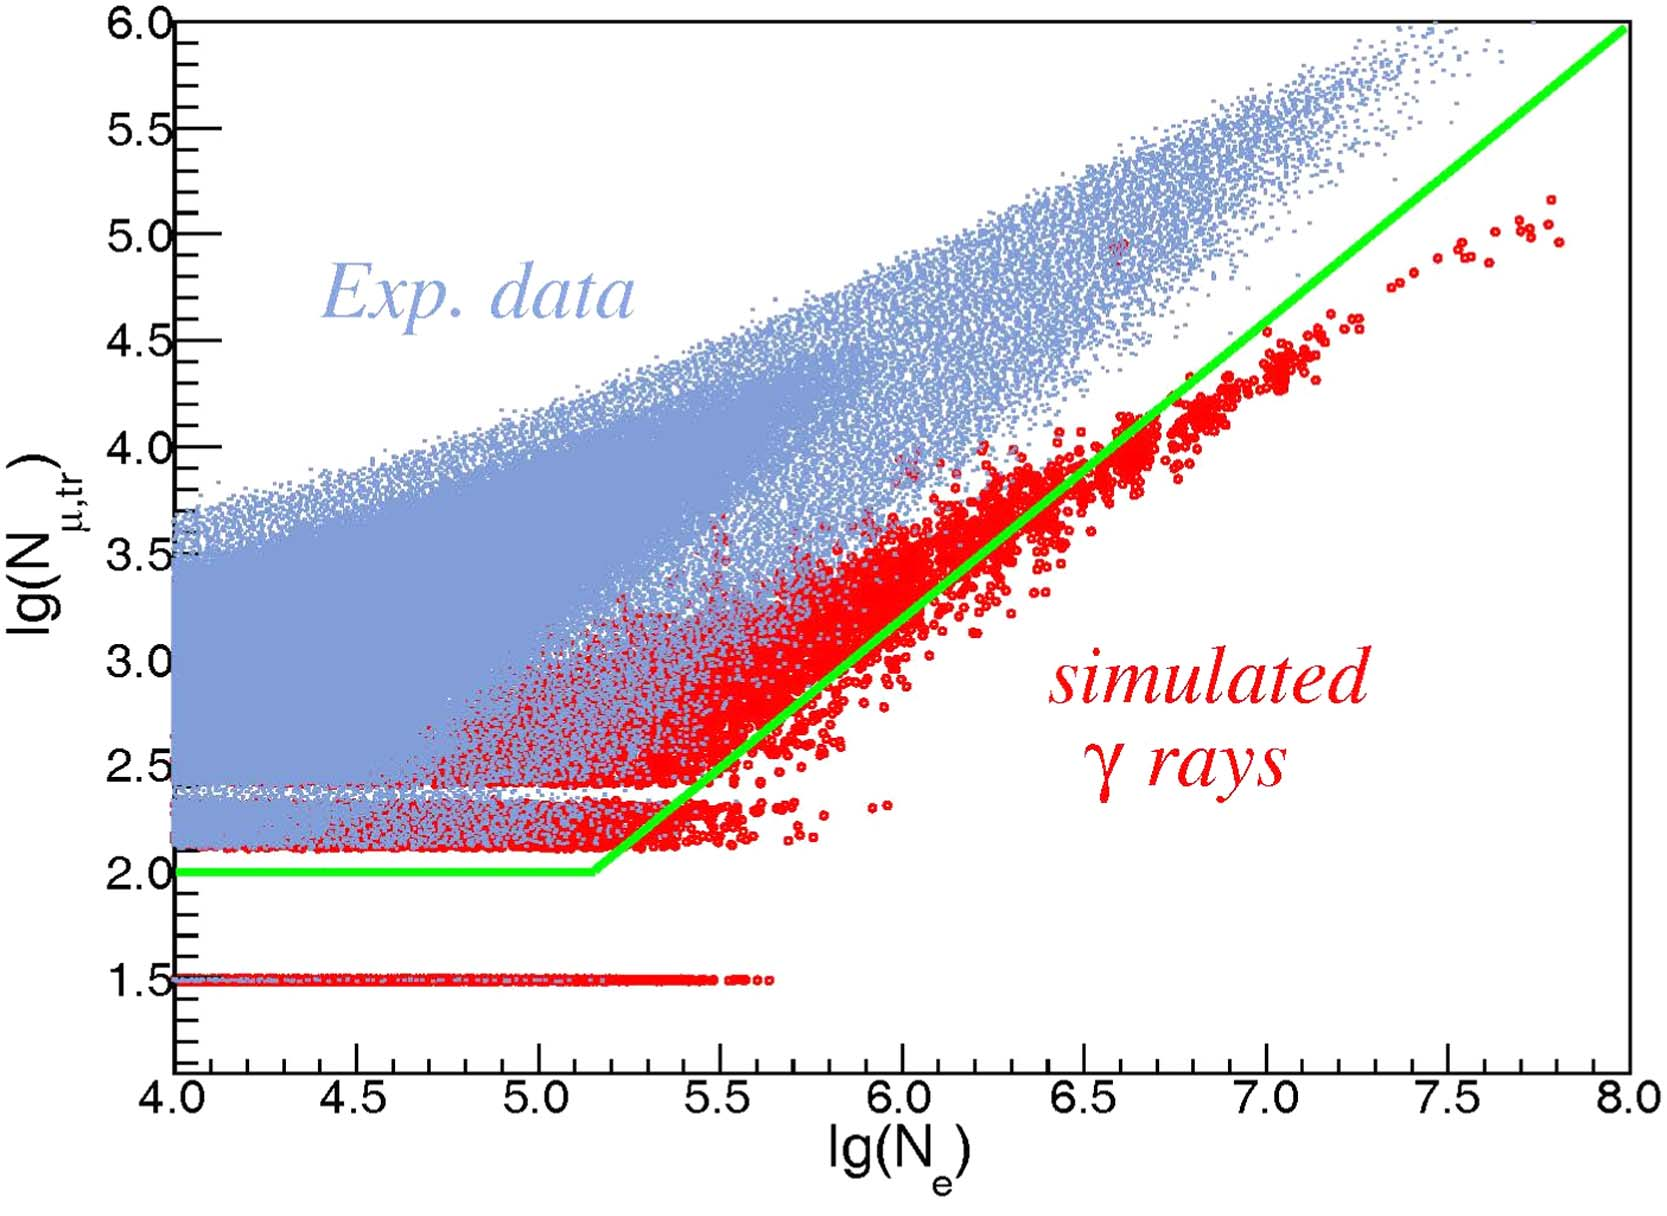
\includegraphics[height=0.39\textheight]{pics/gamma_cut.png}\\
  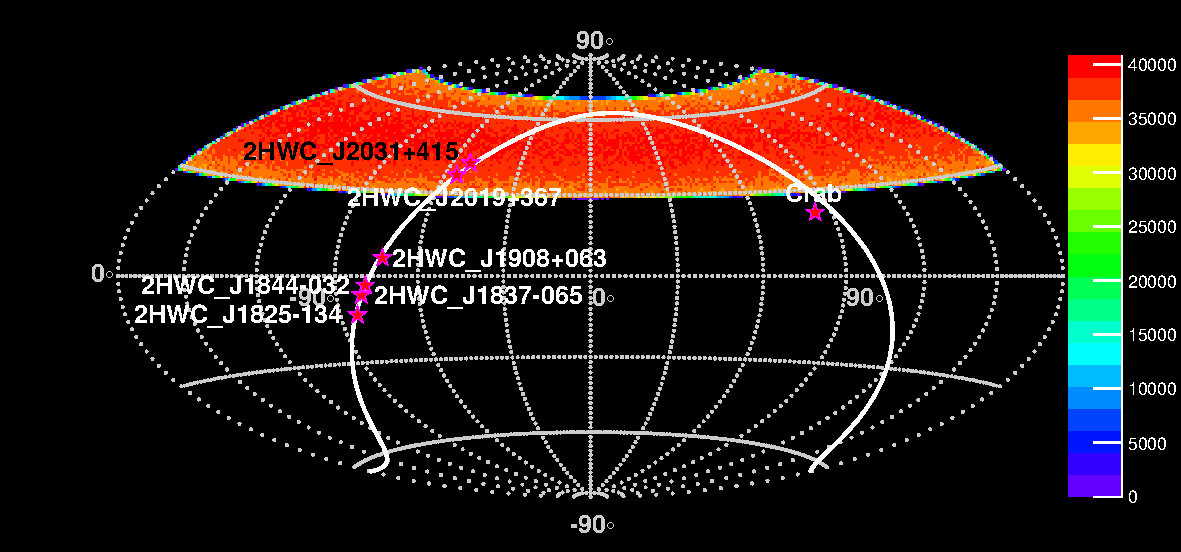
\includegraphics[height=0.42\textheight]{pics/Skymap_6srcs_exp.pdf}
\end{center}
\end{frame}

\begin{frame}{KASCADE-Grande $\gamma$ ray searches}
\begin{itemize}
 \item Limits on the diffuse gamma-ray flux: the best upper limit of the fraction of $\gamma$-rays
to the total cosmic ray flux is obtained at $3.7 \times 10^{15}$~eV and equals $1.1 \times 10^{-5}$. 
\end{itemize}
\begin{center}
  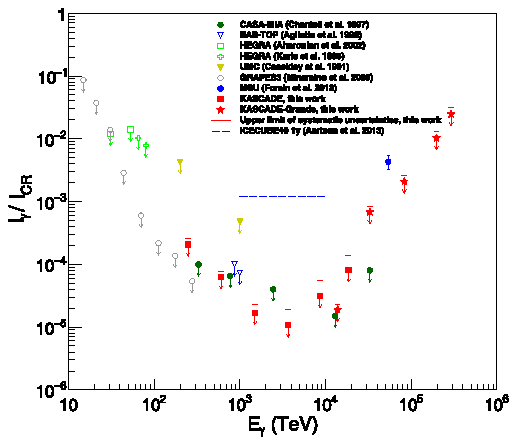
\includegraphics[height=0.56\textheight]{pics/KASCADE-Grande_UHECR2016-1.pdf}
  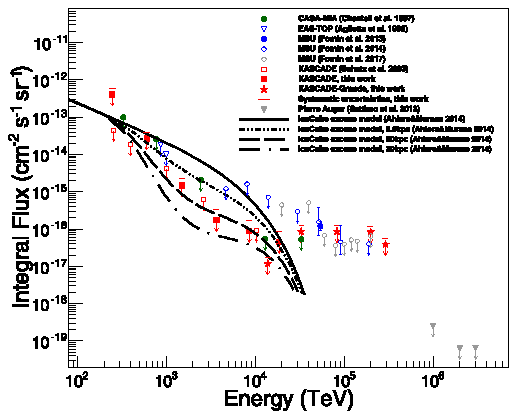
\includegraphics[height=0.56\textheight]{pics/KASCADE-Grande_UHECR2016-2.pdf}
\end{center}
\vspace{-2ex}
\small
[1] W.~Apel et al., \textit{KASCADE-Grande Limits on the Isotropic Diffuse Gamma-Ray Flux between 100~TeV and 1~EeV}, 2017, ApJ, 848, 1.
\end{frame}


\begin{frame}{Flux estimation for the \textit{2HWC\_J2013+415} source}
\[
\Large
\begin{array}{ccc}
E~[\mathrm{TeV}] & N_\gamma & F_\mathrm{int}~[\mathrm{cm}^{-2}\mathrm{s}^{-1}] \\\hline
7 & 441 & 1.4\times10^{-13}\\
56 & 12.9 & 4.1\times10^{-15}\\
100 & 4.8 & 1.5\times10^{-15}\\
1000 & 0.096 & 3.1\times10^{-17}\\
\end{array}
\]
% There supposed to be 2 slides on this
%  Оценка количества событий вокруг 2HWC_J2013+415 +-
\end{frame}
